\documentclass{article}
\usepackage{graphicx} % Required for inserting images
\usepackage{amsfonts}
\usepackage{bm}
\usepackage{amsmath}
\usepackage{booktabs}

\title{24.10.08 Mithril MSP and Benchmark}
\author{Xun Zhang \quad \quad Wuyun Siqin \quad \quad Bingsheng Zhang \\ 
Zhejiang University, CHN \\
22221024@zju.edu.cn \quad 3210101763@zju.edu.cn \quad bingsheng@zju.edu.cn}


\date{October 8 2024}

\begin{document}

\maketitle

\section{Mithril MSP}

There are two versions of $\mathsf{MSP}$ algorithms in the Mithril paper.
We omitted the check of MSP-PoP( a multisignature based on Boneh Lynn Shacham(BLS) signatureswith proofs of possession), since this part will not be included in the relations.


The first one is $\mathsf{MSP.AKey}(\textbf{mvk})$, and $\mathsf{MSP.ASig}(\bm{\sigma})$:


\begin{itemize}
    \item $\mathsf{MSP.AKey}(\textbf{mvk})$: Takes a vector $\textbf{mvk}$ of (previously checked) verification keys and returns an intermediate aggregate public key
    $ivk=\prod mvk_i$
    \item  $\mathsf{MSP.ASig}(\bm{\sigma})$: Takes as input a vector $\bm{\sigma}$ and returns $\mu \leftarrow \prod_{1}^d \sigma_i$,
\end{itemize}

The second one is is $\mathsf{MSP.BKey}(\textbf{mvk}, \bm{e_\sigma})$, and $\mathsf{MSP.BSig}(\bm{\sigma})$:


\begin{itemize}
    \item $\mathsf{MSP.BKey}(\textbf{mvk}, \bm{e_\sigma})$: Takes a vector $\textbf{mvk}$ of (previously checked) verification keys and weighting seed $\bm{e_\sigma}$, and returns an intermediate aggregate public key 
$ivk=\prod mvk_i^{e_i} $, where $e_i \leftarrow \textrm{H}(i,e_\sigma)$.
    \item $\mathsf{MSP.BSig}(\bm{\sigma})$: Takes as input a vector of signatures $\bm{\sigma}$ and returns $(\mu,e_{\bm{\sigma}})$ where
$\mu \leftarrow \prod \sigma_i^{e_i}$, where $e_i \leftarrow \textrm{H}_{\lambda}(i,e_\sigma)$ and $e_\sigma \leftarrow \textrm{H}_{p}(\mathbb{\sigma})$.
\end{itemize}

The reason why Mithril use $\mathsf{MSP.BKey}(\textbf{mvk}, \bm{e_\sigma})$ and $\mathsf{MSP.BSig}(\bm{\sigma})$ is that:
\\
\\
\textit{which enforce more
stringent checking than that of standard multisignatures by utilizing the short random exponent batching of Bellare et al. [5]. The difference from standard multisignature aggregation (via $\mathsf{MSP.AKey}$ and $\mathsf{MSP.ASig}$), is that the randomized
check will fail with overwhelming probability if any of the individual signatures
is invalid, whereas standard aggregation allows for spurious individual signatures
as long as they sum up to the correct aggregate. Furthermore, $\mathsf{MSP.BKey}$ uses a
weighting seed $e_{\bm{\sigma}}$ as input; in practice this is produced by the signature set to be
verified and cannot be run ahead of time. In our use case, this can be overcome by having $\mathsf{MSP.BKey}$ be evaluated inside a proof system.}


\section{Relations for Mithril(latest version)}

Here we post the latest version of Mithril relations(which we plan to prove in SNARK). It is somewhat different from the initial version:

\begin{itemize}
    \item $ivk = \mathsf{MSP.BKey}(\textbf{mvk}, \bm{e_\sigma})$ and $ivk_{\mathsf{body}} = \mathsf{MSP.AKey}(\textbf{mvk})$ 
    \item $(\mu,e_{\bm{\sigma}}) = \mathsf{MSP.BSig}(\bm{\sigma})$
    \item $\forall i : \mathsf{index}_i \leq m$ and $\forall i \neq j : \mathsf{index}_i \neq \mathsf{index}_j$.\item For $i \in \{1 \dots k\}$: $(mvk_i, \mathsf{stake}_i)$ lies in Merkle tree $\mathsf{AVK}, N$ following path $\bm{p}_i$.
    \item For $i \in \{1 \dots k\}$: $\mathsf{MSP.Eval}(\mathsf{topic}, \mathsf{index}_i, \sigma_i) = ev_i$.
    \item For $i \in \{1 \dots k\}$: $ev_i \leq \phi(\mathsf{stake}_i)$.
\end{itemize}

Concretely, statements are $x = (\mathsf{AVK}, ivk, ivk_{\mathsf{body}}, \mu, e_{\bm{\sigma}}, \mathsf{mesg})$ and witnesses are of the form $w = (mvk_i, \mathsf{stake}_i, p_i, ev_i, \sigma_i, \mathsf{index}_i)$ for $i \in \{1 \dots k\}$. 

Note that we implemented the $\mathsf{MSP.vers}(msghash,ivk, \mu)$ in the circuit, so the actually relations will be different from the paper. But we can adjust it for free.


\section{MSP.B Implementation Details}

Here we give the details of $\mathsf{MSP.BKey}$ function.


For $\mathsf{MSP.BKey}(\textbf{mvk}, \bm{e_\sigma})$: Takes a vector $\textbf{mvk}$ of (previously checked) verification keys and weighting seed $\bm{e_\sigma}$, and returns an intermediate aggregate public key.

The code is is as follows:
\\
\\
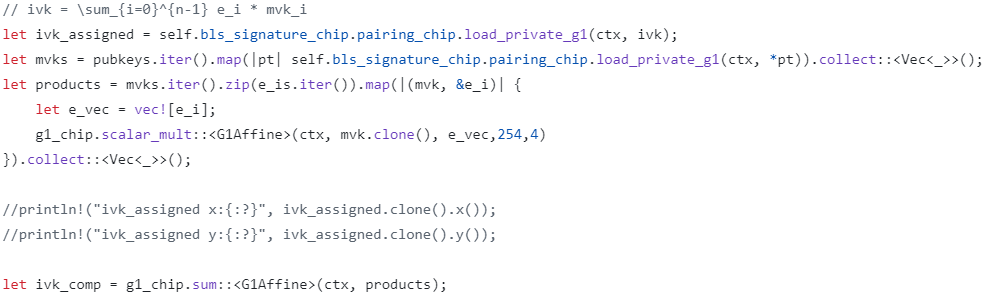
\includegraphics[width=0.9\linewidth]{msp_bkey_ivk_code.png}
\\
\\
For $\mathsf{MSP.BSig}(\bm{\sigma})$: Takes as input a vector of signatures $\bm{\sigma}$ and returns $(\mu,e_{\bm{\sigma}})$ where
$\mu \leftarrow \prod \sigma_i^{e_i}$, where $e_i \leftarrow \textrm{H}_{\lambda}(i,e_\sigma)$ and $e_\sigma \leftarrow \textrm{H}_{p}(\mathbb{\sigma})$.


The code is is as follows:
\\
\\
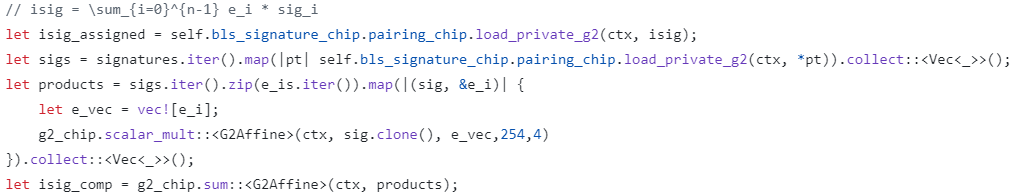
\includegraphics[width=0.9\linewidth]{msp_bkey_isig_code.png}
\\
\\

We use the the method named "scalar\_mult" in halo2-lib. The encapsulated code is as follows:
\\
\\
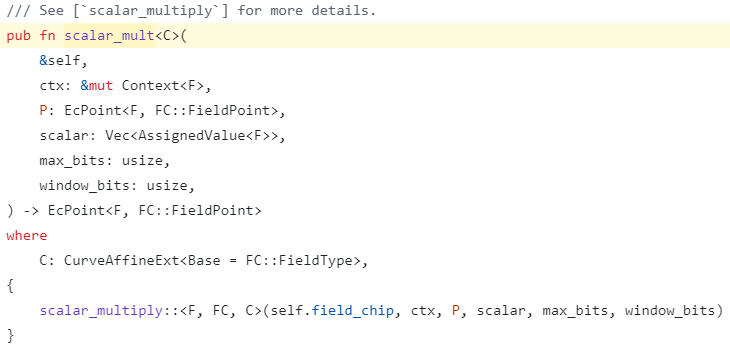
\includegraphics[width=0.9\linewidth]{scalar_mult_code.png}
\\
\\

We use the parameters of this function as follows:

\begin{itemize}
    \item max\_bits: 254. Since we work on the curve BN254, the poseidon function is also on BN254, so the output of hash function is a field element of BN254. We set this to 254 bits, which means the max vlaue of scalar is less than $2^{254}$.

    \item window\_bits: 4. We set the window size of multi-scalar multiplication to 4. Usually this value is set to 2 or 4. Different settings may result in different proving efficiencies, which will be tested later.
\end{itemize}


\section{MSP Benchmark}


\subsection{MSP.A Benchmark}

It is basically a BLS multi-signature, we have benched before, here is the result:


\textbf{Note:} The configuration with Degree , Advice , Lookup , Fixed , Lookup Bits , Limb Bits , Num Limbs is 17, 25, 3, 1, 16, 88, and 3, respectively.

\begin{table}[h]
    \centering
    \begin{tabular}{c|c|c|c} \hline
        Num Aggregation & Proof Time & Proof Size & Verify Time \\ \hline
        2 & 17.4515s & 11520 & 72.7713ms \\ \hline
        200 & 22.3638s & 15008 & 89.0890ms \\ \hline
        2000 & 67.0237s & 45952 & 286.869ms \\ \hline
        4000 & 116.439s & 79680 & 327.100ms \\ \hline
        6000 & 165.035s & 113760 & 551.478ms \\ \hline
        8000 & 210.119s & 147840 & 664.927ms \\ \hline
        10000 & 256.993s & 181920 & 841.507ms \\ \hline
    \end{tabular}
    \caption{Benchmark results for varying aggregation sizes (Version 1)}
    \label{tab:version1_agg}
\end{table}


\subsection{MSP.B Benchmark}

\subsubsection{Server Benchmark}

We benchmarked the $\mathsf{MSP.BKey}$ and $\mathsf{MSP.BSig}$, as well as pairing verification($\mathsf{MSP.Ver}$).

The following benchmark is on the server:

\begin{tabular}{ll}
\textbf{OS} & Ubuntu 20.04.6 LTS (x86\_64) \\
\textbf{Kernel} & 5.4.0-169-generic \\
\textbf{CPU} & Intel Xeon Silver 4214 (48 cores) @ 3.200GHz \\
\textbf{GPU} & 4 x NVIDIA GeForce RTX 2080 Ti \\
\textbf{Memory} & 128546 MiB \\
\end{tabular}
\vspace{1cm}


 \textbf{Note:} The configuration with Degree , Advice , Lookup Bits , Limb Bits , Num Limbs is 19, 6, 18, 90, and 3, respectively.

\begin{tabular}{c|c|c}
\hline
 \text{num\_aggregation} & \text{proving\_time} & \text{verification\_time} \\
\hline
 4   & 70.5080s  & 14.4204ms  \\ \hline
 8   & 100.3936s & 17.5523ms  \\ \hline
 16  & 145.7191s  & 18.6467ms  \\ \hline
 32  & 251.0654s & 21.7318ms  \\ \hline
 64 & 471.5117s & 30.2121ms  \\ \hline
\end{tabular}\\


Our program can only handle signing with up to 64 public keys. When attempting to sign with 128 public keys, the server's 126 GB of RAM and 8 GB swap partition become full, leading to the program being killed. Therefore, the program cannot continue.

\subsubsection{PC Benchmark}

We benchmarked the $\mathsf{MSP.BKey}$ and $\mathsf{MSP.BSig}$, as well as pairing verification($\mathsf{MSP.Ver}$).

The PC's configuration is shown in the following figure.\\

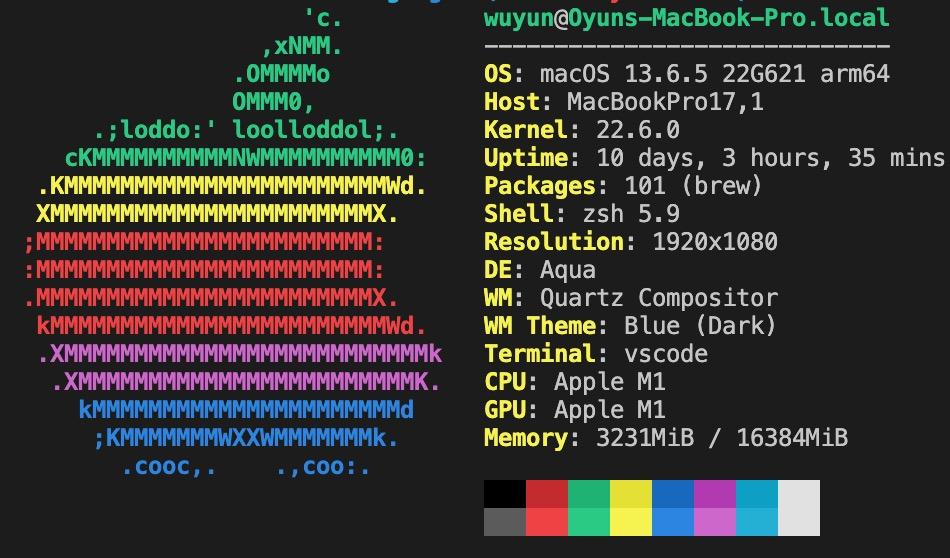
\includegraphics[width=0.9\linewidth]{wuyun_mac.jpg}

The following benchmark is on the PC:\\
\begin{table}[ht]
    \centering
    \begin{tabular}{c|c|c|c|c|c|c|c}
        \toprule  
        num\_advice & degree & lookup\_bits & limb\_bits  & num\_agg  & proving & proof\_size & verification\ \\
        \midrule
        25 & 17 & 16 & 88  & 4   & 73.2230s   & 36192 & 14.5060ms \\
        25 & 17 & 16 & 88  & 8  & 114.6814s  & 49856 & 20.6187ms \\
        6  & 19 & 18 & 90 & 4   & 75.5567s   & 8864  & 5.3844ms  \\
        6  & 19 & 18 & 90  & 8  & 115.3011s    & 12576 & 8.0946ms  \\
        2  & 21 & 20 & 88  & 4   & 118.3032s  & 2848  & 4.2537ms  \\
        2  & 21 & 20 & 88  & 8  & 159.2993s  & 3776  & 5.5756ms  \\
        \bottomrule
    \end{tabular}
    \caption{MSP Benchmark on PC(original)}
    \label{tab:data_table}
\end{table}




We also benchmark the $\mathsf{MSP}$ in the different group, this situation is consistent with the Mithril paper:

\begin{table}[ht]
    \centering
    \begin{tabular}{c|c|c|c|c|c|c|c}
        \toprule
        num\_advice & degree & lookup\_bits & limb\_bits  & num\_agg  & proving & proof\_size & verification \\
        \midrule
        25 & 17 & 16 & 88  & 4   & 73.8717s   & 36192 & 13.4883ms \\
        25 & 17 & 16 & 88  & 8  & 124.6366s  & 49856 & 22.3612ms \\
        6  & 19 & 18 & 90  & 4   & 75.7733s      & 8864  & 5.7507ms   \\
        6  & 19 & 18 & 90  & 8   & 118.0805s  & 12576 & 8.3911ms  \\
        2  & 21 & 20 & 88  & 4   & 117.6121s  & 2848  & 14.2941ms \\
        2  & 21 & 20 & 88  & 8  & 163.3018s   & 3776  & 6.1740ms  \\
        \bottomrule
    \end{tabular}
    \caption{MSP Benchmark on PC(swap group,where pk is on G2)}
    \label{tab:data_table}
\end{table}


Similarly, when we attempt to run 32 signature aggregations on the PC, the 16 GB of RAM and approximately 40 GB of swap partition (which varies) become full, ultimately resulting in the program being killed.

\section{Next Step}

We plan to do more tests and benchmarks on $\mathsf{MSP}$.

\begin{itemize}
    \item Adjust the configs(degree, advice) of $\mathsf{MSP}$ circuit.
    \item Optimize the $\mathsf{scalar\_multi}$ function in halo2-lib.
    \item Manege the RAM on the server to run the large scale data.
\end{itemize}



\end{document}
